\documentclass[10pt]{article}
\usepackage[top=1in, bottom=1.2in]{geometry}
\linespread{1} % line spacing
\geometry{letterpaper}
\usepackage{tabularx}
\usepackage[parfill]{parskip} % begin paragraphs with an empty line rather than an indent
\usepackage[ocgcolorlinks]{hyperref} %ocg coverts links to black when you print -- downside of unbreakable lines



% New command \CustomLabel{labelname} creates a hypertarget and label for referencing
\makeatletter
 \newcommand{\CustomLabel}[1]{\Hy@raisedlink{\hypertarget{#1}{}}\label{#1}}
\makeatother

% Graph Stuff
\usepackage{tikz}
\usetikzlibrary{trees} % this is to allow the fork right path
\usetikzlibrary{calc} % for hyperlinking nodes

% Styling for Graphs
\tikzset{
    basic/.style  = {thin, draw, text width=5em, font=\sffamily, rectangle, minimum size=2em, align=center},
    root/.style   = {basic},
    edge from parent fork down,
        level 2/.style = {basic, grow=down, edge from parent path={(\tikzparentnode.south) |- (\tikzchildnode.west)}},
        level 3/.style = {basic, xshift=1ex,anchor=west},
            subA/.style={level distance=6ex},
            subB/.style={level distance=12ex},
            subC/.style={level distance=18ex},
    hyperlink node/.style={
      postaction={
        path picture={
          \path let
          \p1 = (path picture bounding box.south west),
          \p2 = (path picture bounding box.north east),
          \p3 = (\x2-\x1,\y2-\y1)
          in
          (path picture bounding box.center)
          node[inner sep=0pt,anchor=center,outer sep=0pt]
          {\hyperlink{#1}{\phantom{\rule{\x3}{\y3}}}};
        }
      },
    }
}

\title{\bf Checkers Design Document}
\author{me 3}
\date{}

\begin{document}
\maketitle

\tableofcontents

\section{Introduction}
    This document contains decomposition, uses relationship, and traceability.
    
\section{Modules}
Modules are stuff.

\subsection{Hardware Hiding Module}
    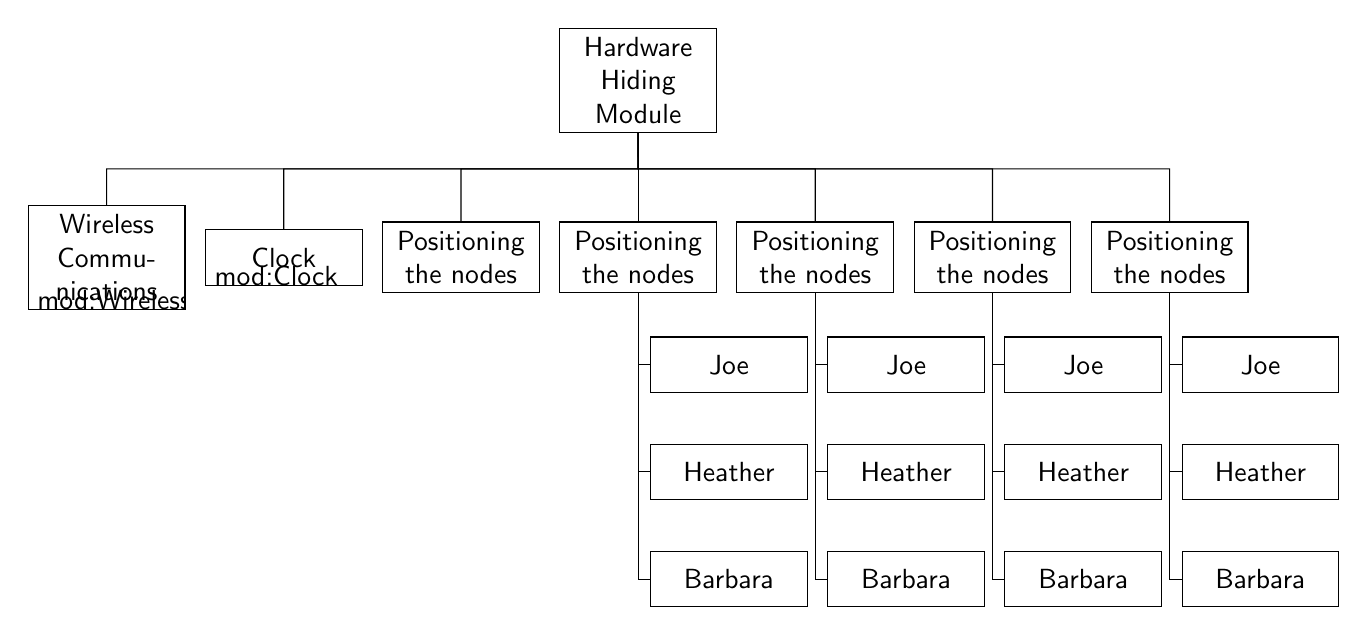
\begin{tikzpicture}[scale=1.5, align=center]
        \node[root] {Hardware Hiding Module}
        child {node[level 2, hyperlink node=mod:WirelessComs]{Wireless Communications}}
        child {node[level 2, hyperlink node=mod:Clock]{Clock}}
        child {node[level 2]{Positioning the nodes}}
        child {node[level 2]{Positioning the nodes}
            child[subA] {node[level 3]{Joe}}
            child[subB] {node[level 3]{Heather}}
            child[subC] {node[level 3]{Barbara}}}
        child {node[level 2]{Positioning the nodes}
            child[subA] {node[level 3]{Joe}}
            child[subB] {node[level 3]{Heather}}
            child[subC] {node[level 3]{Barbara}}}
        child {node[level 2]{Positioning the nodes}
            child[subA] {node[level 3]{Joe}}
            child[subB] {node[level 3]{Heather}}
            child[subC] {node[level 3]{Barbara}}}
        child {node[level 2]{Positioning the nodes}
            child[subA] {node[level 3]{Joe}}
            child[subB] {node[level 3]{Heather}}
            child[subC] {node[level 3]{Barbara}}}
        ;
    \end{tikzpicture}
    
            

    \subsubsection{Wireless Communications Hardware Hiding Module}\CustomLabel{mod:WirelessComs}
        \begin{tabularx}{\linewidth}{ >{\bfseries}r X }
            Type            & Host/Onboard Module \\
            Secret          & This module serves to hide the secret of what wireless communications hardware is being used \\
            Responsibilites & This module is responsible for handling transmission using the wireless communications hardware. \\
            Uses            & None \\
            Design          & None \\
        \end{tabularx}


    \subsubsection{Clock Hardware Hiding Module}\CustomLabel{mod:Clock}
        \begin{tabularx}{\linewidth}{ >{\bfseries}r X }
            Type            & Onboard Module \\
            Secret          & This module serves to hide the secret of what clock hardware is being used. \\
            Responsibilites & This module is responsible for direct monitoring and controlling of the clock hardware. \\
            Uses            & \ref{mod:WirelessComs} \\
            Design          & None \\
        \end{tabularx}
        
\subsection{Behaviour Hiding Module}


\subsection{Software Hiding Module}

    \subsubsection{ TEMPLATE XXX Hiding Module}\label{mod:TEMPLATE}
        \begin{tabularx}{\linewidth}{ >{\bfseries}r X }
            Type            &  \\
            Secret          & Explain why this is an XXX hiding module. \\
            Uses            & \ref{labelhere} \\ % can call row 'Requirements' or 'Uses'
            Code            &  reference to implementation \\ % This row can be called 'Design' or 'Implementation'
        \end{tabularx}
        
\newpage




\section{Module Design}

    \subsection{Wireless Communications Hardware Hiding Module}\CustomLabel{md:WirelessComs}
    \subsubsection{Interface}
        \begin{tabularx}{\linewidth}{ >{\bfseries}r Xp{5cm} }
            Types           & WHAT IS TYPES? It's in page 13 of SE2AA4 design.pdf. \\
            
            Constants       & \begin{tabular}[t]{l l} 
                                     & \\
                                    List off & does magic \\
                                    CONSTANTS & def of what constant does \\
                                    programszzzzzzzzzzzzzzzzzzzzzzzzzzzzz & zzzzzzzzzzzzzzzzzzzzz \\
                                    here & \\ 
                              \end{tabular} \\

            Access Programs & \begin{tabular}[t]{l l} 
                                     & \\
                                    getNumBananas() & Gets int bananas \\
                                    access & def \\
                                    programszzzzzzzzzzzzzzzzzzzzzzzzzzzzz & zzzzzzzzzzzzzzzzzzzzz \\
                                    here & \\ 
                              \end{tabular} \\
                              
        \end{tabularx}
        
    \subsubsection{Implementation}
        \begin{tabularx}{\linewidth}{ >{\bfseries}r Xp{5cm} }
            Types           & WHAT IS TYPES? It's in page 13 of SE2AA4 design.pdf. \\
            
            Constants       & \begin{tabular}[t]{l l} 
                                 & \\
                                List off & does magic \\
                                CONSTANTS & def of what constant does \\
                                programszzzzzzzzzzzzzzzzzzzzzzzzzzzzz & zzzzzzzzzzzzzzzzzzzzz \\
                                here & \\ 
                            \end{tabular} \\
                              
            Variables       & \begin{tabular}[t]{l l} 
                                     & \\
                                    List off & does magic \\
                                    CONSTANTS & def of what constant does \\
                                    programszzzzzzzzzzzzzzzzzzzzzzzzzzzzz & zzzzzzzzzzzzzzzzzzzzz \\
                                    here & \\ 
                              \end{tabular} \\

            Access Programs & \begin{tabular}[t]{l l} 
                                     & \\
                                    \bf{getNumBananas()} & \\
                                    Inputs & None \\
                                    Outputs & NumOfBananas \\
                                    Updates & bananaCount \\ 
                                     & \\
                                    \bf{xxxanas()} & \\
                                    Inputs & None \\
                                    Outputs & NumOfBananas \\
                                    Updates & bananaCount \\ 
                              \end{tabular} \\
                              
        \end{tabularx}
        

\end{document}












